\documentclass[a4paper]{report}

\usepackage[utf8]{inputenc}
\usepackage[T1]{fontenc}
\usepackage[francais]{babel}
\usepackage{graphicx}

\title{Conception d'un accélérateur de calcul de produit scalaire}
\author{Kévin \bsc{Vythelingum} et Jean-Michel \bsc{Nokaya}}
\date{\today}

\begin{document}

\maketitle
\tableofcontents

\chapter*{Introduction}
Dans ce TP, nous réaliserons un accélérateur de calcul de produit scalaire afin tout d'abord de mettre en oeuvre la méthodologie de conception vue en cours, en découpant le système en une unité de contrôle UC et des unités de traitement UTs.
Ensuite, nous programmerons les différentes entités nécessaires en VHDL avant de les intégrer à un projet dans l'environnement de développement Quartus II.
Enfin, l'ensemble sera simulé sur l'outil ModelSim avant d'être exporté et testé sur la carte Altera.

Ce compte-rendu comportera la description de la conception du système, mais aussi une analyse des vues RTL et de la simulation.
L'ensemble des codes commentés se situerons en fin de rapport.

\part{Conception du système}
\chapter{Spécification de l'accélérateur}
On souhaite réaliser un accélérateur matériel pour calculer le produit scalaire de deux vecteurs :

\[
\vec{x}.\vec{y}=\sum_{i=1}^{2}x_{i}y_{i} \mbox{ avec } \vec{x}=\pmatrix{x_{1} \cr x_{2}} \mbox{et } \vec{y}=\pmatrix{y_{1} \cr y_{2}}
\]

Les coordonnées des vecteurs sont des entiers codés sur 4 bits, signés en complément à 2.
Le résultat sera un entier signé codé en complément à 2 sur 8 bits.
L’accélérateur n’intègrera qu’un seul multiplieur et un seul additionneur.
L’accélérateur saura qu’il peut démarrer le calcul (c’est-à-dire que les coordonnées des vecteurs sont disponibles sur ses entrées), lorsqu’un signal départ sera à 1.
L’accélérateur devra fournir en sortie un signal fin qui est à 1 quand le calcul est terminé.
Le signal depart est maintenu à 1 tant que le signal fin n’est pas vu à 1. Ensuite, il repasse à 0 et cela n’est pas immédiat et peut prendre quelques périodes d’horloge.

Sa vue externe sera donc la suivante :

\begin{center}
	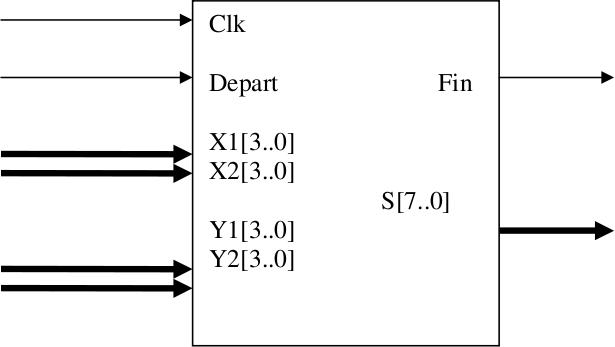
\includegraphics[scale=0.3]{veprod.png}
\end{center}

Le signal Clk est une horloge qui permettra de séquencer l’ensemble.

\chapter{Conception de l'accélérateur}
\section{Les unités de traitement}
Afin de réaliser l'accélérateur matériel, différentes unités de traitement seront nécessaires.
Tout d'abord, les registres d'entrée X1, X2, Y1 et Y2 seront des registres statiques 4 bits à chargement parallèle.
Ensuite, conformément au cahier des charges, nous disposerons d'un multiplieur qui réalisera une multiplication signée en complément à deux, et d'un additionneur.
Enfin, un multiplexeur 2$\times$(2$\times$4 bits) $\rightarrow$ 2$\times$(4 bits) et un registre de sortie statique 9 bits à chargement parallèle et remise à zéro complèteront les UTs.
Le choix de 9 bits pour le registre de sortie est dû à la volonté de pouvoir conserver la retenue éventuelle.
De plus, les unités de traitement synchronisées par le signal d'horloge \emph{clk} sont actives sur front descendant.

L'ensemble des UTs peut être représenté par la figure suivante :

\begin{center}
	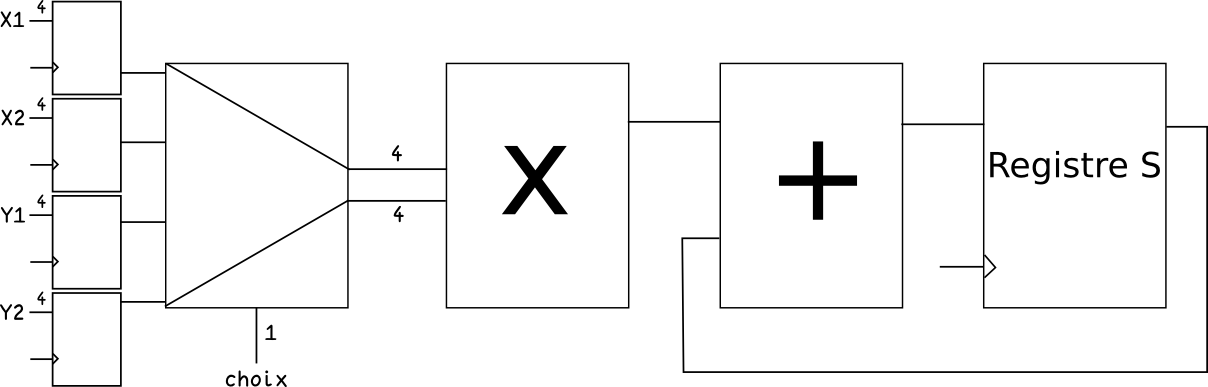
\includegraphics[scale=0.5]{uts.png}
\end{center}

\subsection{Registres d'entrée X1, X2, Y1, Y2}
Ce sont des registres statiques 4 bits à chargement parallèle.
\begin{itemize}
	\item Entrées :
	\begin{itemize}
		\item E[3..0]
		\item load
		\item clk
	\end{itemize}
	\item Sortie :
	\begin{itemize}
		\item S (4 bits)
	\end{itemize}
\end{itemize}

\begin{center}
	\begin{tabular}{|c|c|c|}
		\hline
		clk & load & mode \\
		\hline
		X & 0 & maintien \\
		\hline
		$\downarrow$ & 1 & chargement du registre avec E \\
		\hline
	\end{tabular}
\end{center}

\subsection{Multiplexeur}
C'est un multiplexeur 2$\times$(2$\times$4 bits) $\rightarrow$ 2$\times$(4 bits).
\begin{center}
	\begin{tabular}{|c|c|c|}
		\hline
		choix & Sx & Sy \\
		\hline
		0 & X1 & Y1 \\
		\hline
		1 & X2 & Y2 \\
		\hline
	\end{tabular}
\end{center}

\subsection{Multiplieur}
Il effectue une multiplication signée en complément à deux.
\begin{itemize}
	\item Entrées :
	\begin{itemize}
		\item A (4 bits)
		\item B (4 bits)
	\end{itemize}
	\item Sortie :
	\begin{itemize}
		\item S (9 bits : 8 bits + extension du bit de signe)
	\end{itemize}
\end{itemize}
\[
S <= A*B
\]

\subsection{Additionneur}
\begin{itemize}
	\item Entrées :
	\begin{itemize}
		\item A (9 bits)
		\item B (9 bits)
	\end{itemize}
	\item Sortie :
	\begin{itemize}
		\item S (9 bits)
	\end{itemize}
\end{itemize}
\[
S <= A+B
\]

\subsection{Registre de sortie}
Il s'agit d'un registre statique 9 bits à chargement parallèle et remise à zéro.
Le \emph{load} est prioritaire.
\begin{itemize}
	\item Entrées :
	\begin{itemize}
		\item E[8..0]
		\item load
		\item clear
		\item clk
	\end{itemize}
	\item Sortie :
	\begin{itemize}
		\item S[8..0]
	\end{itemize}
\end{itemize}

\begin{center}
	\begin{tabular}{|c|c|c|c|}
		\hline
		clk & load & clear & mode \\
		\hline
		X & 0 & 0 & maintien \\
		\hline
		$\downarrow$ & 1 & X & chargement parallèle \\
		\hline
		$\downarrow$ & 0 & 1 & mise à zéro \\
		\hline
	\end{tabular}
\end{center}

\section{Le séquenceur}
\subsection{Vue externe de l'UC}
\begin{center}
	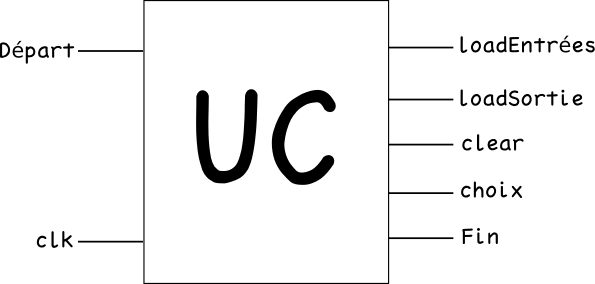
\includegraphics[scale=0.7]{uc.png}
\end{center}
\subsection{Machine d'état}
\begin{center}
	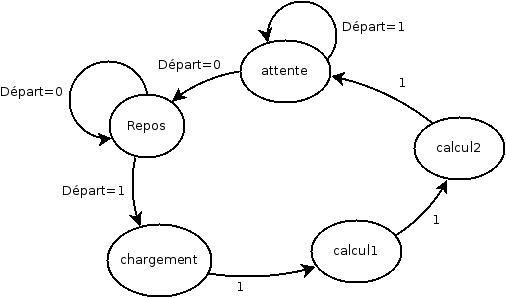
\includegraphics[scale=0.5]{machineEtat.png}
\end{center}

\subsection{Table des sorties en fonction de l'état}
\begin{center}
	\begin{tabular}{|c|c|c|c|c|c|}
		\hline
		état & loadEntrées & loadSortie & clear & choix & Fin \\
		\hline
		repos & 0 & 0 & 0 & 0 & 1 \\
		\hline
		chargement & 1 & 0 & 1 & 0 & 0 \\
		\hline
		calcul1 & 0 & 1 & 0 & 0 & 0 \\
		\hline
		calcul2 & 0 & 1 & 0 & 1 & 0 \\
		\hline
		attente & 0 & 0 & 0 & 0 & 1 \\
		\hline
	\end{tabular}
\end{center}

\part{Programmation VHDL}
\chapter{Unités de traitement}
Dans la répartition des tâches, ce fut Kévin qui se chargea des unités de traitement.

Chaque unité de traitement est accompagnée de sa vue RTL. Il est important de vérifier cette vue afin de s'assurer que le compilateur n'a pas généré de bascules en trop.
\section{Les registres d'entrée}
Le code VHDL est identique pour les quatres registres d'entrée. Une entité \emph{registre} a donc été créée en vue d'être instanciée quatre fois lors de l'intégration dans le projet \emph{produit scalaire}.

La vue RTL d'une instance de registre est la suivante :
\begin{center}
	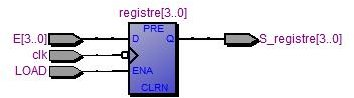
\includegraphics[scale=1]{registre_instance1_registre1.jpg}
\end{center}
On reconnaît la bascule qui constitue notre registre. De manière générale, cette vue est identique à la réprésentation théorique en vue externe de notre registre.
\section{Le multiplexeur}
Le code VHDL du multiplexeur est celui fourni dans le tutoriel de familiarisation à l'environnement de développement Quartus II.
Il a suffit de le compiler et de créer un symbole à partir du fichier pour l'inclure au projet \emph{produit scalaire}.

La vue RTL du multiplexeur est la suivante :
\begin{center}
	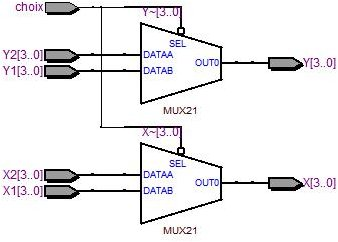
\includegraphics[scale=1]{mux_instance_mux.jpg}
\end{center}
On retrouve deux multiplexeur 2$\times$(4 bits) $\rightarrow$ 1$\times$(4 bits) qui constituent notre multiplexeur 2$\times$(2$\times$4 bits) $\rightarrow$ 2$\times$(4 bits).
\section{Le multiplieur-accumulateur}
L'ensemble composé du multiplieur, de l'accumulateur et du registre de sortie est réalisé à partir d'une unique entité VHDL appelée \emph{mac}.
En effet, il est possible de regrouper ces UTs dans une même entité car elles répondent à une unique équation logique :
\[
S = X*Y+S
\]
La vue RTL du multiplieur-accumulateur est la suivante :
\begin{center}
	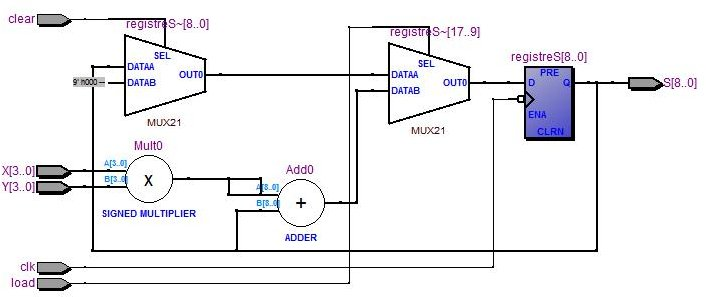
\includegraphics[scale=0.7]{mac_instance_mac.jpg}
\end{center}
On a bien une seule bascule pour notre registre de sortie. Les deux multiplexeurs correspondent aux \emph{if} du code VHDL.
\chapter{Unité de contôle}
Dans la répartition des tâches, ce fut Jean-Michel qui se chargea de l'unité de contrôle.

Pour constituer l'UC, il a suffit de décrire son comportement en VHDL.
Le fait d'avoir conçu une machine d'état accompagnée de sa table des sorties en fonction de l'état auparavant facilite ce travail dans la mesure où cela n'est plus qu'un exercice de traduction.

La vue RTL de l'ensemble de l'unité de contrôle est la suivante :
\begin{center}
	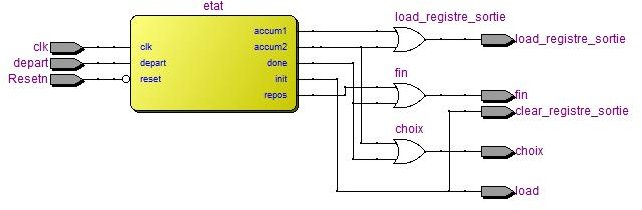
\includegraphics[scale=0.7]{uc_instance_uc.jpg}
\end{center}
On retrouve la vue externe théorique précédente.
Les portes \bsc{ou} représentent les deux étapes de calcul nécessaires au calcul du produit scalaire.
\chapter{Test-bench}
\section{Intégration dans le projet \emph{produit scalaire}}
Avant de réaliser le test-bench à proprement parler, il a fallu intégrer l'ensemble des composants dans un même projet \emph{produit scalaire}.
Dans un premier temps, nous avons réalisé l'intégration en mode schéma, c'est-à-dire que nous avons connecté les différents composants directement à partir de leur représentation schématique.
Cependant, la compilation du schéma n'a pas engendré un code VHDL compilable pour effectuer la simulation.
De fait, il a été décidé de réaliser à nouveau l'intégration des composants, mais cette fois directement en VHDL.

La vue RTL de l'ensemble du projet est la suivante :
\begin{center}
	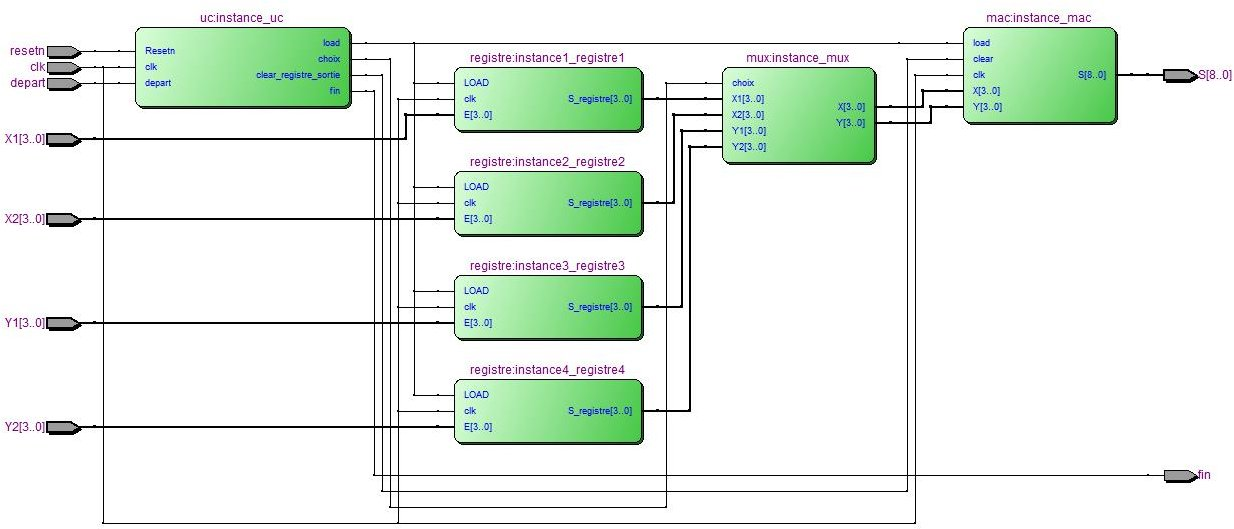
\includegraphics[scale=0.4]{produitscalaire1.jpg}
\end{center}

\section{Réalisation du test-bench}
Le test-bench permet de simuler les actions que peut effectuer l'utilisateur directement sur la carte.
Dans notre cas, il s'agit de générer un processus d'horloge pour simuler le signal \emph{clk}, de générer un signal \emph{Départ} et de décider des valeurs des registres d'entrée comme pourrait le faire un utilisateur via les switch de la carte.

\part{Simulation et test}
\chapter{Simulation avec ModelSim}
La simulation avec ModelSim se lance depuis Quartus. En effet, on indique a Quartus le simulateur ModelSim et le test-bench à utiliser, et ModelSim compile le test-bench avant de lancer la simulation.

Pour vérifier que le système conçu fonctionne, il est nécessaire d'ajouter les signaux de toutes les unités aux signaux mis par défaut afin de contrôler leur comportement.
On ajoute ainsi les signaux de départ, des registres d'entrée et de sortie et de la machine d'état.

Lors du premier test, la machine d'état n'avançait pas, c'est-à-dire qu'elle restait dans l'état \emph{repos}.
Le problème a été réglé en ajoutant le signal \emph{départ} à la liste de sensibilité des signaux de l'UC dans son code VHDL.

Après recompilation, le système fonctionnait globalement mais en regardant dans les détails on s'est aperçu que le signal du registre de sortie restait en \emph{undefined}.
Une première solution était de passer le \emph{load} à 0 au lieu de 1 dans le code de l'UC au moment de l'initialisation, en pensant que le problème venait du fait que comme le registre de sortie se chargeait à partir de son état précédent, il fallait d'abord le mettre à 0.
Cependant, la simulation suivante a montré que la sortie restait à 0 indéfiniment après ce changement, sans qu'aucun calcul ne s'effectue.

Ayant comparé notre code à celui de Fabien et Hugo, nous n'avons pas trouvé de différences mis à part le fait que leur simulation validait leur système.
Nous avons donc effectué le test sur la carte avec leur système.
\chapter{Test sur la carte Altera}
Pour tester le système sur la carte, il suffit d'envoyer le code dessus via USB puis de mettre des valeurs sur les switchs pour observer le résultat sur les LED.
Le signal d'horloge est généré manuellement en appuyant sur un bouton poussoir.

Afin de mettre en oeuvre le système, nous avons calculé le produit scalaire de $\vec{x}=\pmatrix{2\cr0}$ et $\vec{y}=\pmatrix{2\cr0}$ puis de $\vec{x}=\pmatrix{2\cr3}$ et $\vec{y}=\pmatrix{2\cr4}$.

Le test sur la carte s'est révélé concluant.

\chapter*{Conclusion}
En somme, le différentes étapes (conception, programmation, simulation, test) conduisent bien et sont toutes indispensables à la réalisation du système.
De plus, on peut dire que c'est la phase de conception qui est déterminante pour toute la suite. On en conclut qu'il est préférable de passer du temps sur cette partie.

On pourra retenir que le test-bench est propre à la simulation et qu'il ne faut donc pas le compiler à partir de Quartus (qui ne comprend pas les instructions \emph{wait} par exemple), mais l'indiquer à ModelSim.
Aussi, l'intégration des composants du système en VHDL directement est à préférer à celle en mode schéma.

Concernant l'état d'avancement du projet, nous sommes parvenu jusqu'à la simulation du système mais n'arrivant pas à trouver la deuxième erreur dans notre code, nous avons effectué le test sur la carte avec un autre groupe.

\part{Codes commentés}

\end{document}
